\section{Definitions of Limits}

We begin with the definition of the limit of a function.

\begin{thm}{Limit of a Function}
  Consider the function $f$, defined at all $x$ around some value $a$ except possibly at $a$ itself.
  If $f(x)$ is arbitrarily close to the single real number $L$ whenever $x$ is sufficiently close to, but not equal to, $a$, then we say that the limit of $f$ is $L$ as $x$ approaches $a$, and we write
  \[\lim_{x\to a} f(x) = L\]
  Alternatively, we can write that $f(x)\to L$ when $x\to a$.
\end{thm}

We note that in this definition, we do not actually consider $f(a)$.
In fact, the function value at $x=a$ doesn't even have to exist.
We only care about the function values \textit{around} the point at $x=a$.

When we investigate limits, we'll do so in three different ways:\footnote{
These three methods of investigation will remain consistent for most new concepts we discuss in this text.}
\begin{enumerate}
  \item Numerically
  \item Graphically
  \item Analytically
\end{enumerate}

In this section, we will discuss some numerical and graphical approximations of limits, and will build up to analytical evaluations of a limit in the next few sections.

\section*{Numerical Approximations}

Consider the function $f(x) = x-4$.

Let's say we want to investigate the behavior of the function\footnote{We're mainly interested in whether or not there's a specific $y$-value that the function is arbitrarily close to.} \textit{around} $x=2$.
What are the function values doing around that point?
When $x$ is sufficiently close to $2$, is $f(x)$ arbitrarily close to some single real number?

If I were to ask you these questions, how would you approach answering them?

Let's start by just picking some $x$-values that are ``close to'' $2$.
What $x$-values are you thinking of?

Let's start with $x=1.5$.
We can find $f(1.5)$ pretty easily:
\begin{align*}
  f(1.5) & = 1.5-4\\
  & = -2.5
\end{align*}

Our predicament now is that we are trying to see what $y$-value (if any), this is arbitrarily close to.
We don't really hanve enough evidence to say right now.
Maybe we need an $x$-value that is \textit{closer} to $2$.

Let's try $x=1.9$.
\begin{align*}
  f(1.9) & = 1.9-4\\
  & = -2.1
\end{align*}

We might have an idea now of what $f(x)$ is close to.
We can always try this again, maybe with $x=1.99$ now.
\begin{align*}
  f(1.99) & = 1.99-4\\
  & = -2.01
\end{align*}

We can keep this going a bit more:

\begin{center}
  \begin{tabular}{cccccc} \toprule
    $\bm{x}$ & 1.5 & 1.9 & 1.99 & 1.999 & 1.9999\\ \midrule
    $\bm{f(x)}$ & $-2.5$ & $-2.1$ & $-2.01$ & $-2.001$ & $-2.0001$\\ \bottomrule
  \end{tabular}
\end{center}

So, do we have a good idea of what real number $f(x)$ is getting arbitrarily close to when $x$ is sufficiently close to $2$?\footnote{Here's something to think about: why not just start with $x=2$? Go back to the definition of a limit and see.}

It should be obvious in this case: it looks like $f(x) \to -2$ when $x\to 2$.
We have some good evidence that $\dlim_{x\to 2}x-4 = -2$.

But wait, is this ok? We've tried to look at $x$-values that were sufficiently close to $2$, but we've only looked at $x$-values that are \textit{less than} 2.
Why not repeat this process with $x$-values that are close to, but slightly larger than, 2?

\begin{center}
  \begin{tabular}{cccccc} \toprule
    2.0001 & 2.001 & 2.01 & 2.1 & 2.5 & $\bm{x}$\\ \midrule
    $-1.9999$ & $-1.999$ & $-1.99$ & $-1.9$ & $-1.5$ & $\bm{f(x)}$ \\ \bottomrule
  \end{tabular}
\end{center}

Well this is good news! It still looks like $f(x) \to -2$ when $x\to 2$.
We probably have enough evidence to believe that $\dlim_{x\to 2}(x-4) = -2$.

Maybe more importantly, though, we've touched on a very important concept with limits.

\subsection*{One-Sided Limits}

We've seen already, then, that there are two ``sides'' to a limit, since we can look at values of $x$ that are \textit{close to} $a$ on either side: $x$-values that less than $a$, and $x$-values that are greater than $a$.\footnote{We use the terminology ``left'' and ``right'' because of the number line: values less than $a$ on a number line are on the left of $a$, and values greater than $a$ on the number line are on the right of $a$.}

\begin{defn}{Right-Sided Limit}
  If $f$ is arbitrarily close to the single real-number $L$ whenever $x$ is sufficiently close to, but greater than, $a$, then we write:
  \[ \lim_{x\to a^+} f(x)=L\]
\end{defn}

\begin{defn}{Left-Sided Limit}
  If $f$ is arbitrarily close to the single real-number $L$ whenever $x$ is sufficiently close to, but less than, $a$, then we write:
  \[ \lim_{x\to a^-} f(x)=L\]
\end{defn}

In our example above, whether we looked at $x$-values that were slightly less than $2$ or $x$-values that were slightly greater than $2$, the function values seemed to be getting arbitrarily close to $-2$.
Since both the right-sided limit and the left-sided limit were the same, we decided that we had more than enough evidence to conclude that the limit of the function as $x$ approached $2$ was $-2$.

What would we have concluded if the one-sided limits did not match?

\begin{thm}{The Existence (and Non-Existence) of a Limit}
  If $f$ is some function defined at all $x$-values on either side of $a$ except possibly at $a$ itself and $L$ is some real number, then we say that $\dlim_{x\to a} f(x) = L$ if and only if $\dlim_{x\to a^-}f(x) = L$ and $\dlim_{x\to a^+} f(x) = L$.

  If $\dlim_{x\to a^-} f(x) \neq \dlim_{x\to a^+} f(x)$, then we say that $\dlim_{x\to a} f(x)$ does not exist.
\end{thm}

\subsection*{Another Example}

Let's approximate $\dlim_{x\to -3} x^2+1$ numerically.

\textbf{Left-Sided Limit}

\begin{tabular}{ccccc} \toprule
  $\bm{x}$ & $-3.5$ & $-3.1$ & $-3.01$ & $-3.001$ \\ \midrule
  $\bm{f(x)}$ & $13.25$ & $10.61$ & $10.0601$ & $10.006001$\\ \bottomrule
\end{tabular}

\begin{flushright}
  \textbf{Right-Sided Limit}

  \begin{tabular}{ccccc} \toprule
    $-2.999$ & $-2.99$ & $-2.9$ & $-2.5$ & $\bm{x}$ \\ \midrule
    $9.994001$ & $9.9401$ & $9.41$ & $7.25$ & $\bm{f(x)}$ \\ \bottomrule
  \end{tabular}
\end{flushright}

Likely this enough for us to believe that $f(x) \to 10$ when $x\to -3$, or $\dlim_{x\to-3} (x^2+1)=10$.

We'll see some more examples of numerical approximation near the end of this section, but first let's look at things graphically.

\section*{Graphical Approximations}

With graphical approximations, we're essentially going to repeat the process that we've done for numerical approximations.
The main difference is in the representation of the function.

When we had the function represented in some algebraic expression ($f(x) = ...$), we could approximate the limit $\dlim_{x\to a} f(x)$ by evaluating our function at $x$-values.
We picked $x$-values that were ``sufficiently close'' to $a$ on either side, and tried to figure out what the corresponding $y$-values were ``arbitrarily close'' to.

In this context, though, we'll have functions represented graphically.
We still want to evaluate our functions at a bunch of $x$-values and find the corresponding $y$-values.
But now, instead of plugging those $x$-values into an algebraic rule or expression, we'll be looking at a picture of a graph to find those $y$-values.

Consider this function $f(x)$, graphed below.

\begin{figure}[h!tb]
  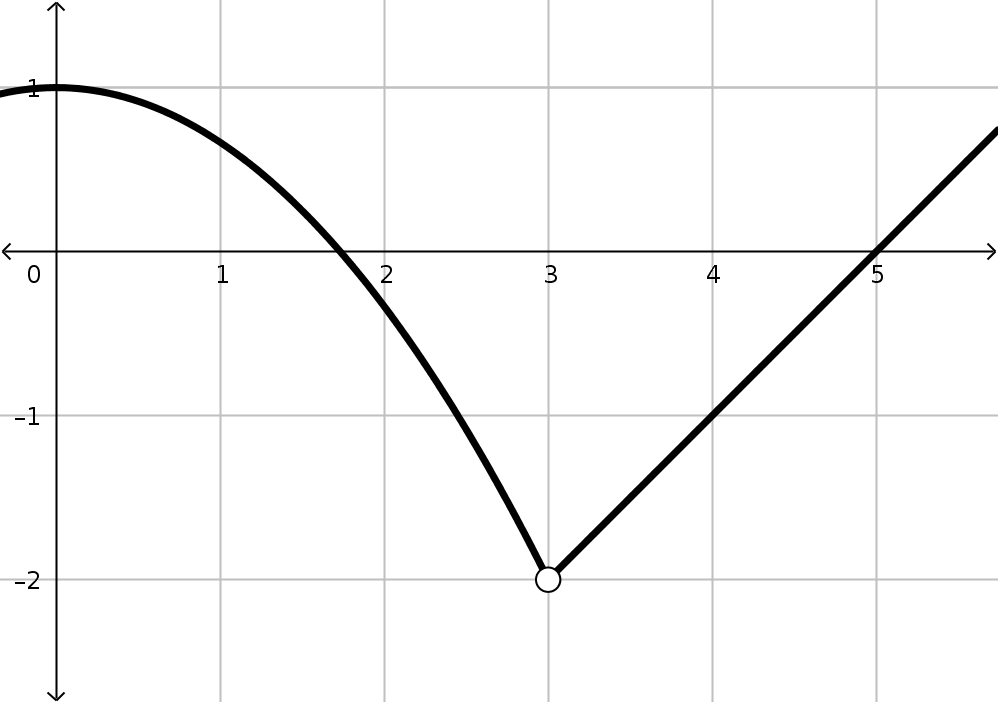
\includegraphics[scale=0.75]{./1_limits/images/1-1_graph1.png}
  \centering
\end{figure}

If we look at the limit $\dlim_{x\to 3} f(x)$, we can try to evaluate our function near $3$.
Instead of actually evaluating it, though, we'll have to look at the $y$-values from the graph.

\textbf{Left-Sided Limit}

When we approximate the left-sided limit, we can pick some points on the graph that are ``on the left'' of $x=3$.
You can see these plotted in red.

\begin{figure}[h!tb]
  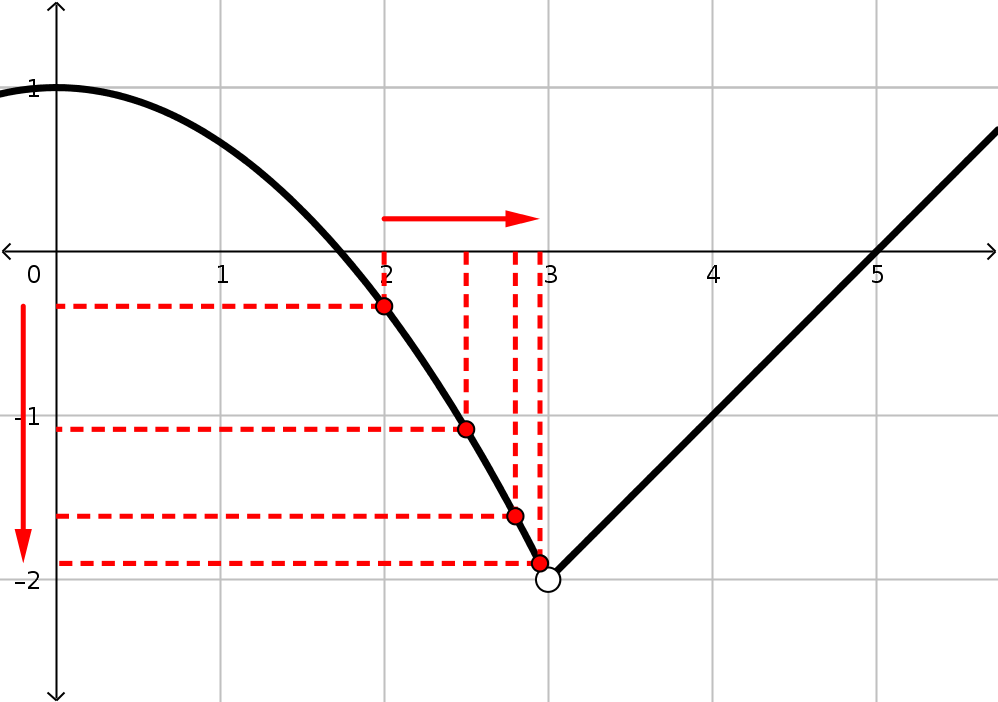
\includegraphics[scale=0.75]{./1_limits/images/1-1_graph1L.png}
  \centering
\end{figure}

Try to follow the movement on the red points as the $x$-values increase up to $3$.
Remember, when we're approximating a limit, we're trying to find what $y$-value we're getting aribtrarily close to.
As we follow the movement of the red points, we can see that the $y$-values drop.
What are they approaching?

Graphically, then, it looks like as $x\to 3^-$, $f(x) \to -2$.
We can say we've got evidence that $\dlim_{x\to 3^-} fx) = -2$.

\textbf{Right-Sided Limit}

Let's do the same thing on the right.
We'll pick some points, plotted in blue this time\footnote{In your own practice, find a way of visualizing these points -- draw arrows, plot points, draw movement, etc. Find something that works for you!}, and try to follow the movement of the $y$-values.

\begin{figure}[h!tb]
  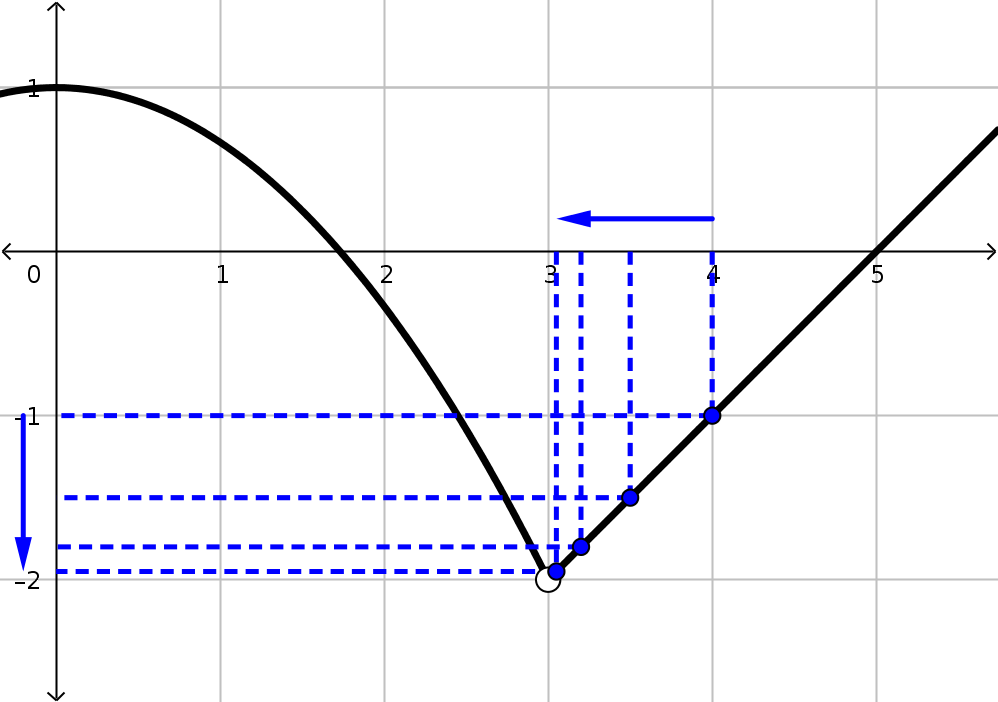
\includegraphics[scale=0.75]{./1_limits/images/1-1_graph1R.png}
  \centering
\end{figure}

So here, based on the graph, it looks like as $x\to 3^+$, $f(x)\to -2$.
Likely, then, we believe that $\dlim_{x\to 3^+} f(x) = -2$.

So we have graphical evidence that $\dlim_{x\to 3^-} f(x) = \dlim_{x\to 3^+} f(x) = -2$.

Graphical approximations are typically nice\footnote{Don't get too nervous! It normally takes students a little bit to be able to read a graph quickly and easily. Go slowly and build that intuition!} to work with and fast to do.
With this visual medium, we can get a ton of information quickly just by glancing at our graph.
We can get approximations on both of the one-sided limits.

This time, then, instead of taking the time to plot all of those points on each side individually, we'll use the graph to see the behavior of the function around $x=3$.
Focus on an interval of $x$-values around $3$.

\begin{figure}[h!tb]
  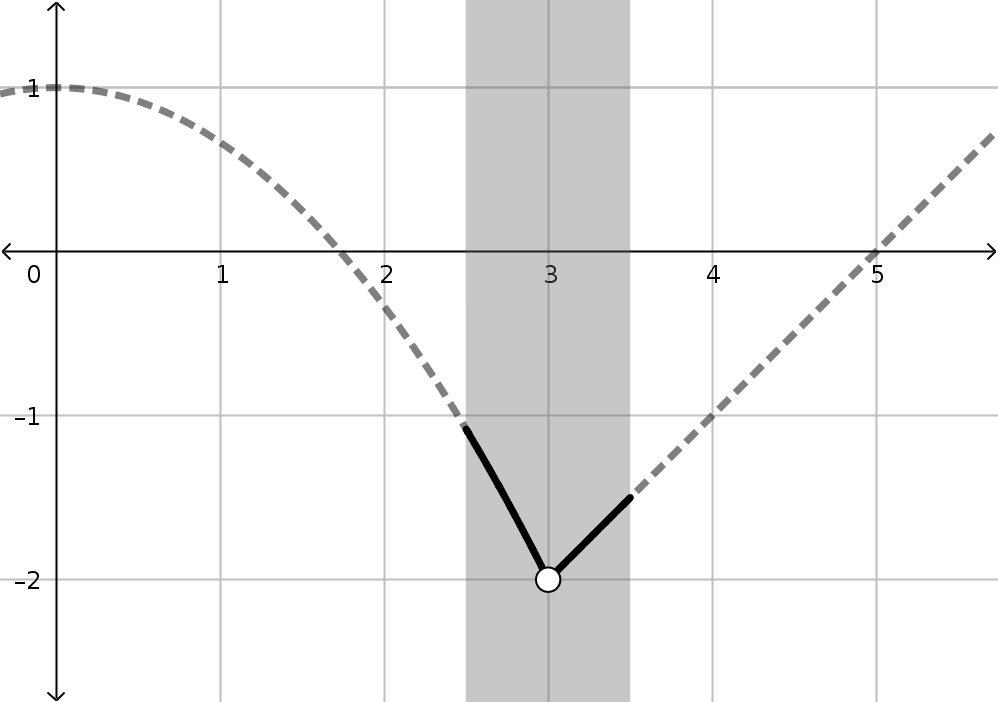
\includegraphics[scale=0.75]{./1_limits/images/1-1_graph1bar1.png}
  \centering
\end{figure}

Look at the graph behavior in this interval.
What is the function doing on either side of $x=3$?
What are the $y$-values close to?

If it's hard to tell, let's consider a smaller interval of $x$-values.

\begin{figure}[h!tb]
  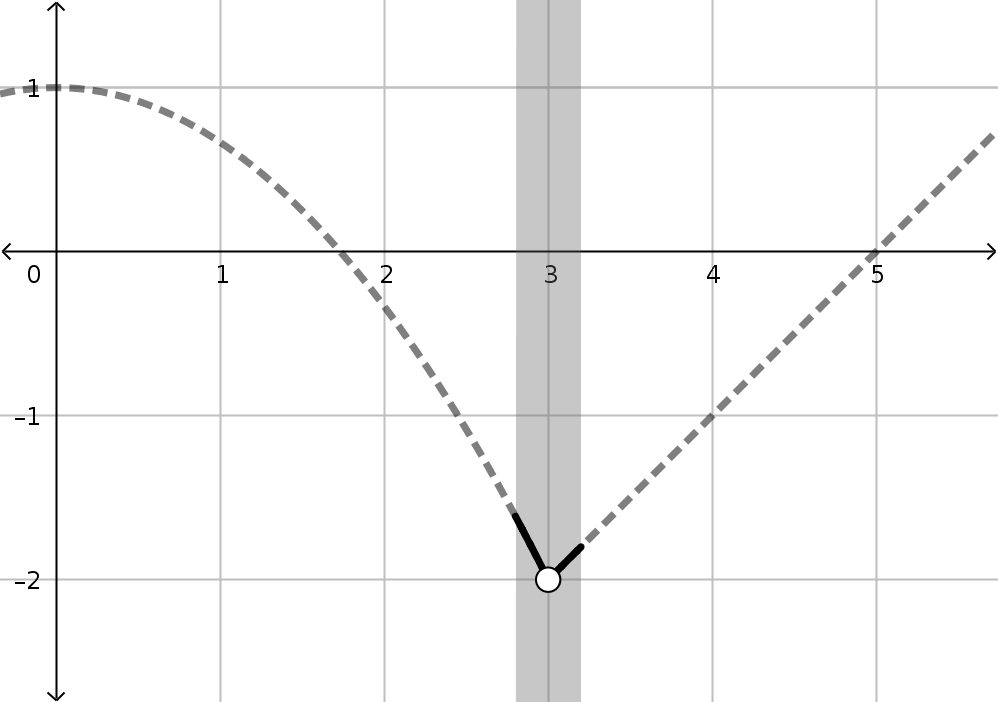
\includegraphics[scale=0.75]{./1_limits/images/1-1_graph1bar2.png}
  \centering
\end{figure}

Hopefully we can see that around $x=3$, the $y$-values on the graph are all close to $-2$.
We have the same behavior on both sides.
In this ``interval'' visualization, we can easily see that the graph seems to be ``going'' to the same $y$-value on both sides of $x=3$.

Let's use this method to approximate another limit. Consider the function $g(x)$, graphed below.
We'll try to approximate the limit $\dlim_{x\to-1} g(x)$.

\begin{figure}[h!tb]
  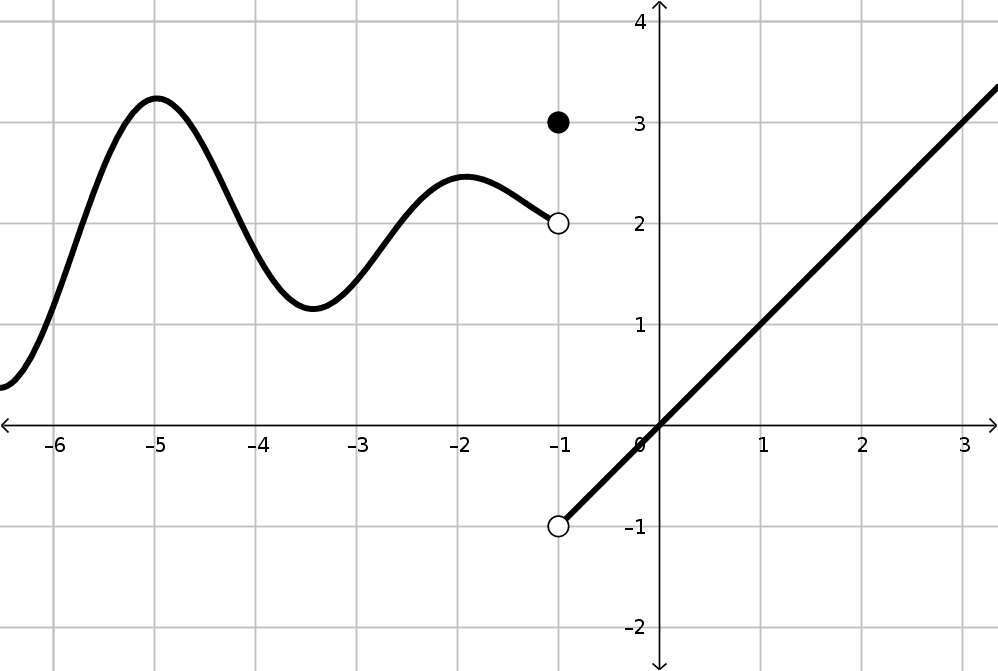
\includegraphics[scale=0.75]{./1_limits/images/1-1_graph2.png}
  \centering
\end{figure}

Let's again focus on an interval of $x$-values around $-1$, and try to talk about the behavior of the function on either side of $x=-1$.

\begin{figure}[h!tb]
  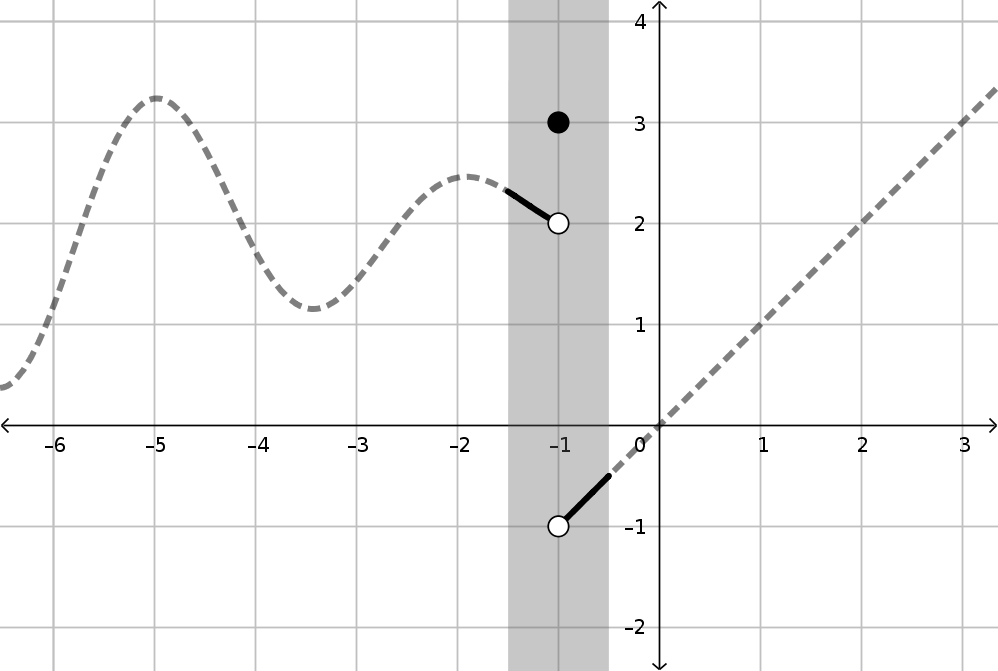
\includegraphics[scale=0.75]{./1_limits/images/1-1_graph2bar1.png}
  \centering
\end{figure}

Notice that there are three things happening:
\begin{enumerate}
  \item On the left of $x=-1$, the $y$-values on the graph seem like they're close to $y=2$.
  \item On the right of $x=-1$, the $y$-values on the graph seem like they're close to $y=-1$.
  \item At $x=-1$ specifically, we have $g(-1)=3$.
\end{enumerate}

Remember that with limits, we only care about the function \textit{around} (but not at) the specific $x$-value.
So in this case, the fact that $g(-1)=3$ is not relevant at all.
All we're concerned with is the limit of the function as $x$ \textit{approaches} $-1$.

So the other two things we noticed really give us our limit statements.

Visually, it looks like $\dlim_{x\to -1^-} g(x) = 2$, but $\dlim_{x\to -1^+} g(x) = -1$. Thus, since we have evidence that $\dlim_{x\to -1^-} g(x) \neq \dlim_{x\to -1^+} g(x)$, we should probably conclude that the limit $\dlim_{x\to -1} g(x)$ does not exist.

\section*{A Warning}

Hopefully we can see how these numerical and graphical approximations are helpful in building some intuition about whether a limit exists or not, and what it may be.

Remember though, these are just approximations!
\begin{defn}{Numerically}
  We can definitely see in the example above that even when we were pretty sure that the limit existed, it may be hard to tell exactly what it is.
  It could also be possible that the limit doesn't exist, because the left-sided limit and the right-sided limit are very similar but not actually the same.\\

  For instance, what if $\dlim_{x\to a^-} f(x) = 1.98325678$ and $\dlim_{x\to a^+} f(x) = 1.98325635$.
  It would be very hard to notice this difference numerically.
  We might (wrongly) conclude that the left-sided limit and right-sided limits are both $1.983256$\footnote{Notice how quickly we gave up on the numerical approximations for the examples above before we just concluded that the one-sided limits probably matched up.}, and then (mistakenly) say that $\dlim_{x\to a} f(x)=1.983256$ instead of saying it doesn't exist.
\end{defn}

\begin{defn}{Graphically}
  Imagine a similar situation as above, but we only get to look at the picture of the graph.
  If $\dlim_{x\to a^-} f(x) = 1.98325678$ and $\dlim_{x\to a^+} f(x) = 1.98325635$, we would likely not notice.
  On any normal scale, the difference between the $y$-value $1.98325678$ and the $y$-value $1.98325635$ would be imperceptible.\\

  Also, even if we're pretty sure that a limit might exist, if that limit doesn't fall on a ``nice'' value (like an integer, or some other value that matches up with the $y$-axis scale), then we may not be able to tell what it is.
\end{defn}

We must approach these approximations with a grain of salt -- these approximations aren't perfect.
They are, however, very helpful.
We can gain valuable insight and build intuition about limits through these approximations.
Putting both of these approximation methods together for the same problem gives us a well-rounded view of the limit we're investigating, and a good amount of evidence for either existence or non-existence.

We'll practice this in these next few examples.

\section*{Examples}


\begin{enumerate}
  \item Let's approximate $\dlim_{x\to 2} \dfrac{x-4}{\sqrt{x}-2}$.

  \textbf{Left-Sided Limit}

  \begin{tabular}{ccccc} \toprule
    $\bm{x}$ & $1.5$ & $1.9$ & $1.99$ & $1.999$ \\ \midrule
    $\bm{f(x)}$ & $3.2247449$ & $3.3784049$ & $3.4106736$ & $3.4138600$\\ \bottomrule
  \end{tabular}

  \begin{flushright}
    \textbf{Right-Sided Limit}

    \begin{tabular}{ccccc} \toprule
      $2.001$ & $2.01$ & $2.1$ & $2.5$ & $\bm{x}$ \\ \midrule
      $3.4145671$ & $3.4177447$ & $3.4491377$ & $3.5811388$ & $\bm{f(x)}$ \\ \bottomrule
    \end{tabular}
  \end{flushright}

  Hopefully we're seeing the problem with approximations: it is not clear what the exact value of the $y$-value that we're getting close to is.
  It looks like it's approximately 3.41(ish), but that's not great.
  We'd like to get an exact value here!

  You also might notice that this is the first example that isn't ``obvious:'' in all of the other examples, we could have just evaluated the function at the $x$-value we were considering.
  Here, though, if $f(x) = \dfrac{x-4}{\sqrt{x}-2}$, we can see that $f(2)$ is not defined.
  Strangely, though, it does look like the limit should exist -- the left-sided limit and the right-side limit look to be the same, although we can't easily tell what they are exactly.

  Let's look at the graph.

  \begin{figure}[h!tb]
    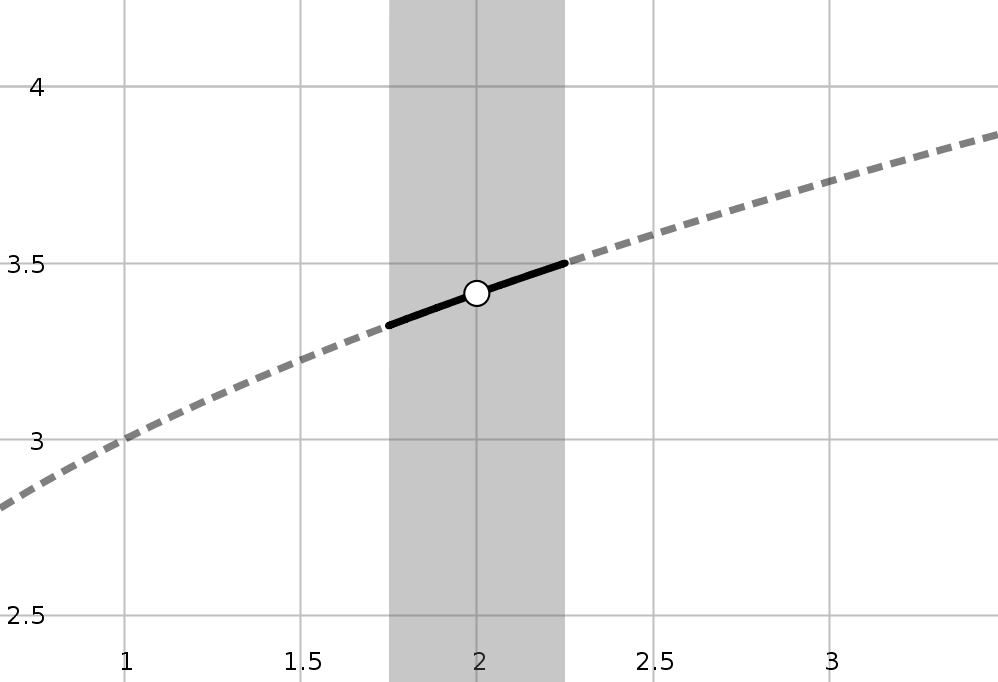
\includegraphics[scale=0.75]{./1_limits/images/1-1_graph3.png}
    \centering
  \end{figure}

  Again, we have some pretty convincing evidence that the limit exists, but it is difficult to see what it actually is.
  Since the $y$-values aren't approaching one of the values used for the scale (i.e. one of the grid lines), we can only guess at what the $y$-value that the graph is approaching actually is.

  \item Let's approximate $\dlim_{x\to 1} \dfrac{|x-1|}{x-1}$.

  We'll start things off with some numerical estimates:

  \textbf{Left-Sided Limit}

  \begin{tabular}{ccccc} \toprule
    $\bm{x}$ & $0.5$ & $0.9$ & $0.99$ & $0.999$ \\ \midrule
    $\bm{f(x)}$ & $-1$ & $-1$ & $-1$ & $-1$\\ \bottomrule
  \end{tabular}

  \begin{flushright}
    \textbf{Right-Sided Limit}

    \begin{tabular}{ccccc} \toprule
      $1.001$ & $1.01$ & $1.1$ & $1.5$ & $\bm{x}$ \\ \midrule
      $1$ & $1$ & $1$ & $1$ & $\bm{f(x)}$ \\ \bottomrule
    \end{tabular}
  \end{flushright}

  Very strange!
  In fact, this doesn't really feel like \textit{approximation} at all, since there doesn't seem to be much guess-work involved in figuring out which $y$-value is being approached.

  Let's confirm our suspicions graphically.

  \begin{figure}[h!tb]
    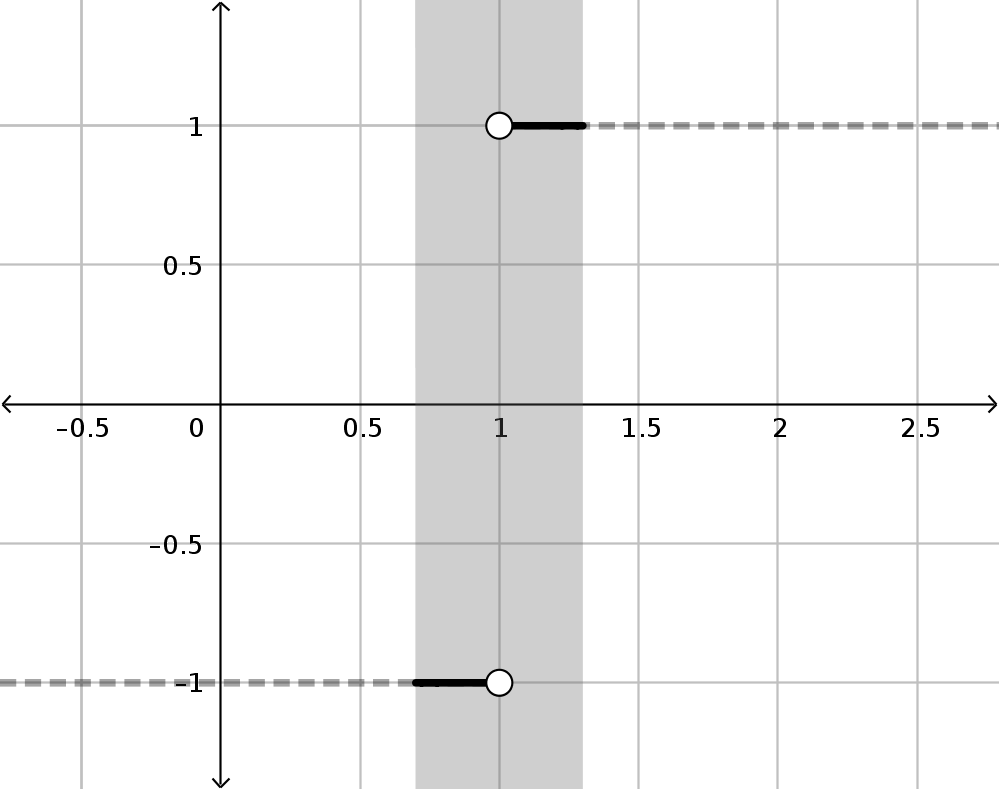
\includegraphics[scale=0.75]{./1_limits/images/1-1_graph4.png}
    \centering
  \end{figure}

  Sure enough, it's easy to see what's going on with this limit:

  $$\dlim_{x\to1^-} \dfrac{|x-1|}{x-1} = -1 \hspace{2cm}\dlim_{x\to1^+} \dfrac{|x-1|}{x-1} = 1$$

  So we likely believe that $\dlim_{x\to1} \dfrac{|x-1|}{x-1}$ does not exist, since the left-sided limit and the right-sided limit do not agree.\footnote{Can you explain what is happening here in general?
  Can we evaluate these one-sided limits without appealing to a graph or some test points?
  What, exactly, is that absolute value doing, and why does the behavior change on one side of $x=1$ compared to the other?

  These are good questions to think about and answer to yourselves.}
\end{enumerate}

\section*{So How Can We Do Better Than Approximations?}

We've seen the benefits and drawbacks of approximations of limits.
We should be thinking about how we might push past this idea of approximation and into \textit{evaluation}.
How can we tell exactly what a limit is without having to rely on test points or graphs?
For the examples when we \textit{do} have test points and graphs, but we still don't know exactly what the limit is, what do we do then?

We can use an example to push towards limit evaluation, and also to notice another kind of non-existence.

\subsection*{Last Example}

Examine $\dlim_{x\to 0} \sin(1/x)$ numerically and graphically.

I won't write out the number approximations, because you'll notice that they're wildly different depending on what $x$-values you pick that are close to $0$ (on either side).

Strange.

Let's investigate the graph of $f(x) = \sin(1/x)$ around $x=0$.

\begin{figure}[h!tb]
  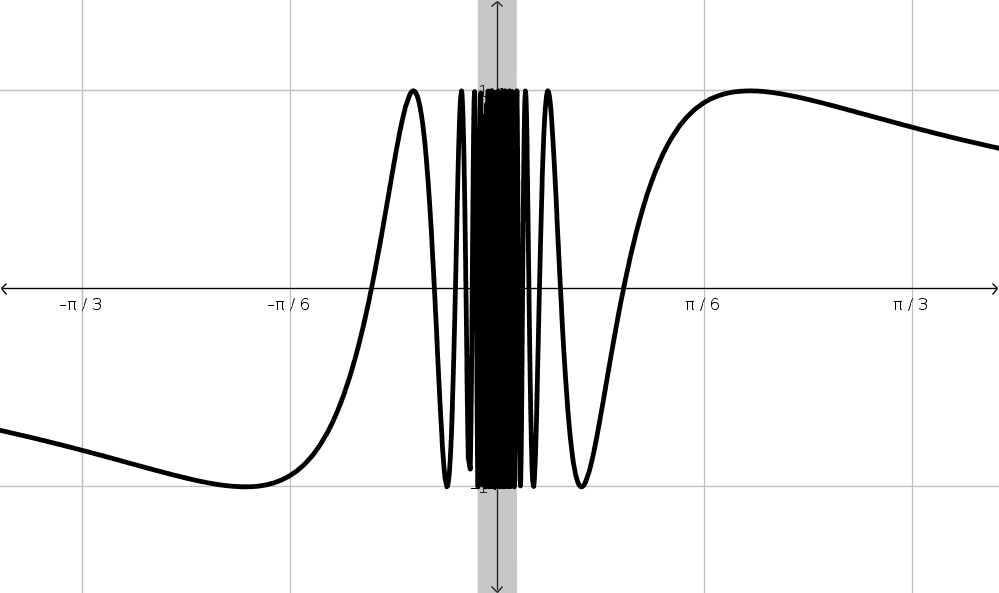
\includegraphics[scale=1]{./1_limits/images/1-1_graph5.png}
  \centering
\end{figure}

This is no help at all. We could try to zoom in further, but that dark, dense, mess of a function around $x=0$ won't clear itself up.
Let's instead try to get an idea of how to analyze the limit without approximations.

First, let's nail down one of the things we're seeing graphically: the range of $f(x) = \sin(1/x)$ is $[-1,1]$.
This is because the range of $\sin\theta$ is $[-1,1]$, and in this case we're just saying that $\theta = \frac{1}{x}$.

Second, notice that the domain of $f(x) = \sin(1/x)$ is $(-\infty,0)\cup(0,\infty)$. We cannot evaluate $f(0)$, since we'd be trying to find $\sin(1/0)$ and $1/0$ is not a real number.
This isn't a huge deal for us, though, because we can remember: we're trying to find $\dlim_{x\to0} \sin(1/x)$, which does not rely on the function value at $x=0$.
We only care about the function values \textit{around} $x=0$.

Let's figure out what happens around $x=0$.
For no specific reason, let's just look at the right-sided limit first: $\dlim_{x\to 0^+} \sin(1/x)$.

Above, we looked at a kind of variable substitution: if $\theta = 1/x$, then $\sin(1/x) = \sin \theta$.
So if $x\to 0^+$, What's happening to $\theta$?
Notice that as we divide 1 by smaller and smaller values, the value of $1/x$ gets larger and larger.
Since $x>0$ (since it's a right-sided limit), $\theta = 1/x$ is getting larger in the positive direction.

So really, then, the question can be re-phrased: instead of trying to figure out what $\sin(1/x)$ approaches as $x$ approaches $0$ on the right, we can think about trying to understand the behavior of $\sin \theta$ as $\theta$ gets larger and larger.

We can understand this behavior in two ways:
\begin{enumerate}
  \item Think of the graph of $y=\sin\theta$:
  \begin{figure}[h!tb]
    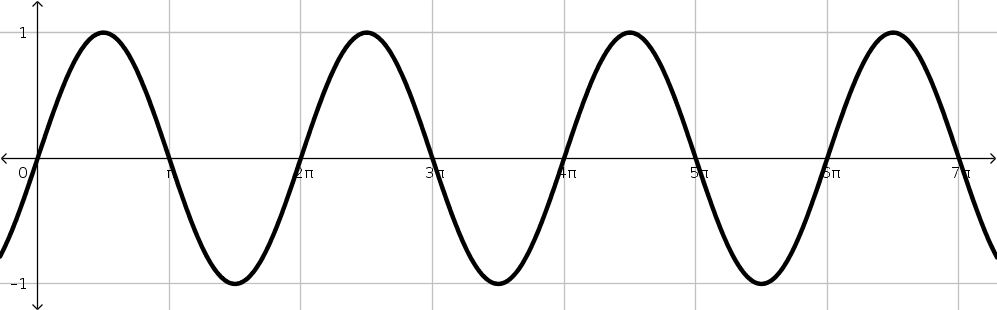
\includegraphics[scale=1]{./1_limits/images/1-1_graph6.png}
    \centering
  \end{figure}
  We can see that as $\theta$ gets larger, $\sin\theta$ just keeps oscillating between $-1$ and $1$ over and over.
  \item Think about the unit circle:
  \begin{figure}[h!tb]
    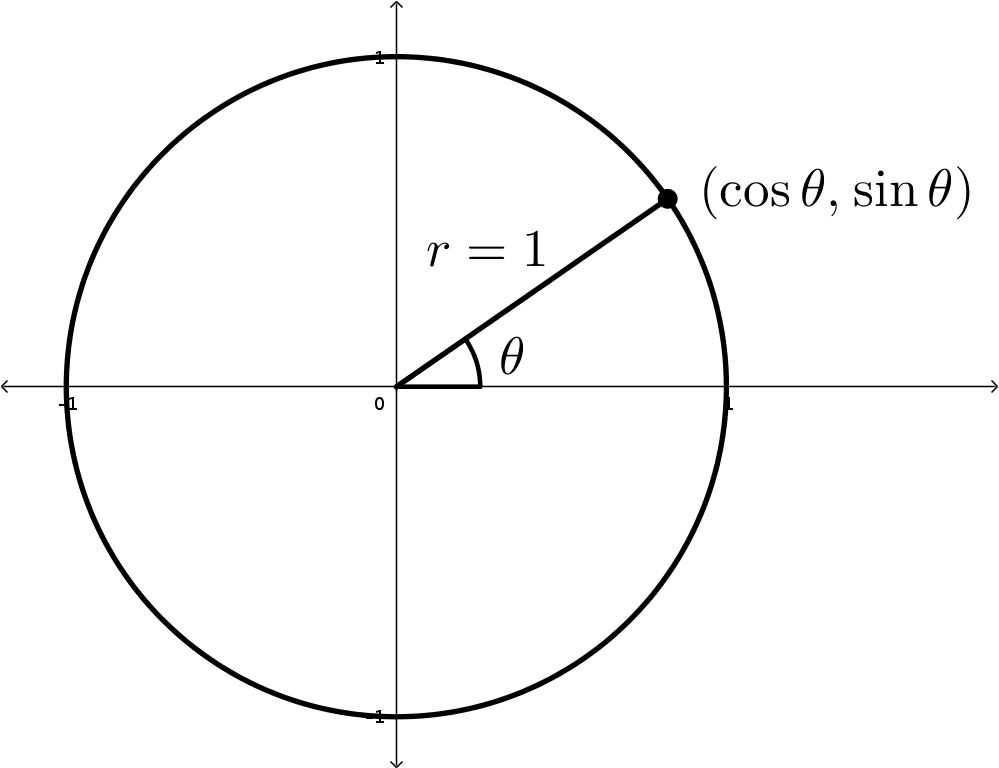
\includegraphics[scale=1]{./1_limits/images/unitcirc.png}
    \centering
  \end{figure}
  We can see that as $\theta$ increases, our point will move around the unit circle in a counterclockwise rotation.
  Since $\sin\theta$ defines the vertical component of the point (the $y$-value on the unit circle), we can see that the highest $y$-value our point will have is $1$.
  Similarly, the lowest $y$-value our point can have is $-1$.
  So as $\theta$ increases, we again see that $\sin\theta$ keeps oscillaring back and forth between $-1$ and $1$.
\end{enumerate}

If we think about the definition of a limit, that means that we \textit{don't} have a single real number $L$ that our function, $\sin\theta$ gets arbitrarily close to as $\theta$ gets larger and larger.
If there's not that single real number, then our limit does not exist.

So all of this to say: as $x\to 0^+$, $\sin(1/x)$ oscillates between $-1$ and $1$, and does not approach a single real number.
So $\dlim_{x\to 0^+} \sin(1/x)$ doesn't exist.

So what about $\dlim_{x\to 0^-} \sin(1/x)$?
You should be able to see almost the exact same thing happening, except that we're looking at the angle $\theta$ getting very negative.
Still, though, we'll find that the oscillation of the $\sin\theta$ function is going give us this non-existent limit.

So then $\dlim_{x\to0} \sin(1/x)$ doesn't exist.
Not because the left and right-sided limits don't match up.
Instead, the limit doesn't exist because the one-sided limits don't exist, and they don't exist because there is not a single real number that $\sin(1/x)$ approaches.

This kind of analysis is less about number crunching and more about thinking about the function behavior.
We'll begin doing that more and more, now.
In the next sections, we'll build up some properties of limits and functions that will allow us to think about and evaluate limits relatively quickly.
